\documentclass{beamer}
\usepackage{graphicx, epstopdf}
\usepackage{amsmath, amssymb, amsbsy, amstext}
% \usepackage{xcolor}

\usepackage[utf8]{inputenc}
\usepackage{natbib}

\usepackage{todonotes}
% \usepackage[disable]{todonotes}
\presetkeys{todonotes}{inline}{}

\usepackage{booktabs}               % for much better looking tables
\usepackage{tabularx}

% \definecolor{darkgreen}{rgb}{0,0.6,0}
% \usepackage{pgf}
% \logo{\pgfputat{\pgfxy(-2,6)}{\pgfbox[center,base]{\includegraphics[height=2cm]{amsilogo.jpg}}}}

\usetheme{Darmstadt} 
%\usetheme{Dresden} %Dresden, Darmstadt, Warsaw
% \usecolortheme{dove}
\title{Sphere Detection using Boosted Classifiers}
% \subtitle{Computer Vision Interim Report}
\author{Brendan Annable, Mitchell Metcalfe, Monica Olejniczak}
\institute{The University of Newcastle, Australia}
\date{\today}

\begin{document}

	\maketitle

	\section{Motivation}
	
	% \begin{frame}{Object detection}
	% 	\begin{center}
			
	% 		To create an object detector using supervised learning, a correctly
	% 		labelled dataset needs to be created for training.

	% 		\citet{opencv_library}

	% 	\end{center}
	% \end{frame}

	% Title slide

	% Motivation:
	%   - ball detection for robot soccer
	%   - Robocup
	%     - need to know where the ball is
	%     - circle detection
	%       * common problems:
	%         - centre circle
	%         - penalty spots
	%         - line intersections
	%         - anything that looks round from some angle
	%   - Possible solutions:
	%     - Classify the texture of the desired object
	%     - train a generic sphere classifier and use it to detect the ball
	%         - potential wider appeal

	% Focus of work
	%	- Detect spheres
	%   - do not detect other 'round things'
	%   (show example images)

	% Literature

	% Methodology
	%  (describe the goal of comparing techniques)

	% Training

	% Results

	% Conclusion

	% References


	\begin{frame}{Bibliography}
		\bibliography{references}
    	\bibliographystyle{apalike}
	\end{frame}

\end{document}


% 	\begin{frame}{Manual labelling}

% 		\begin{itemize}
% 			\item Tedious
% 			\item Error prone
% 			\item Ambiguous
% 		\end{itemize}

% 		% \begin{center}
			
% 		% 	This is a tedious and error prone process, as each object
% 		% 	typically needs to be manually labelled by having a human draw a
% 		% 	rectangle around it.
			
% 		% 	The exact position and dimensions that these rectangles should be
% 		% 	can be ambiguous, as objects may appear in differing orientations
% 		% 	and deformations.

% 		% \end{center}
% 	\end{frame}

% 	\begin{frame}{Example application}
% 		\begin{center}
% 			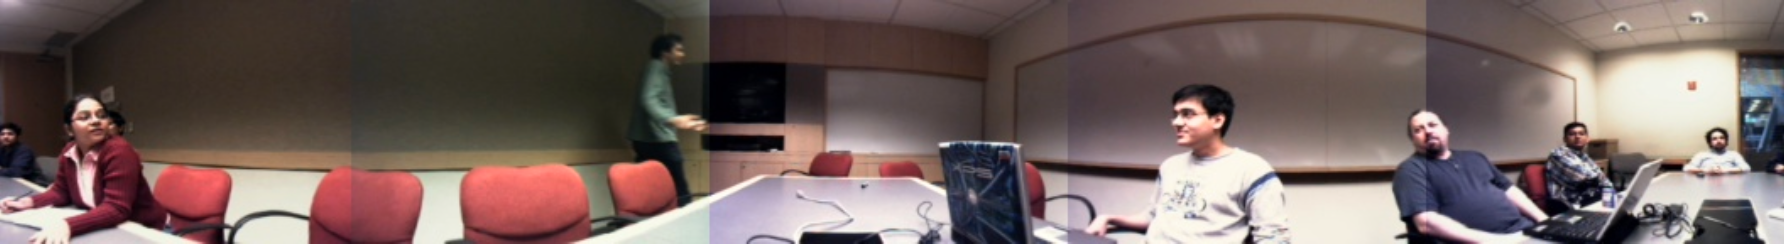
\includegraphics[width=1\textwidth]{input-1.png} \\
% 			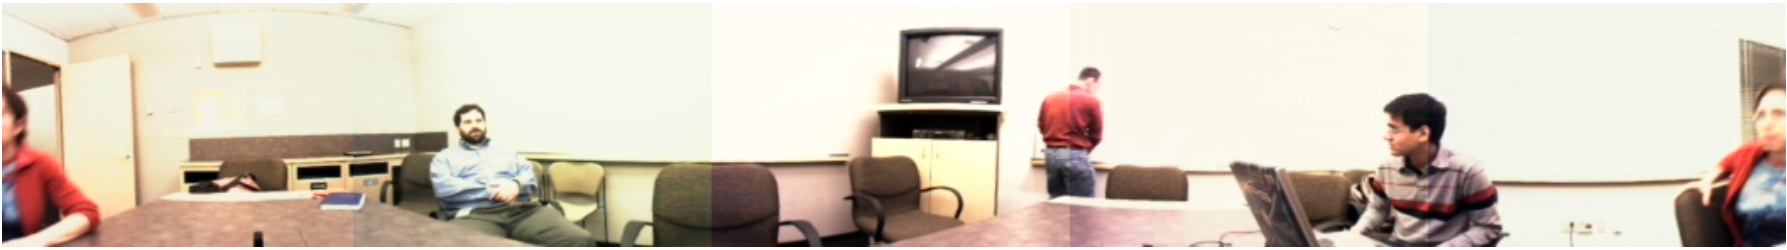
\includegraphics[width=1\textwidth]{input-2.png}
% 		\end{center}
% 	\end{frame}

% 	\begin{frame}{Example application}

% 			Harder than face detection:

% 			\begin{itemize}
% 				\item People can face away from the camera
% 				\item Faces are small
% 				\item Context is required for detection
% 				\item How much context should be used?
% 			\end{itemize}

% 			% This problem is harder than face detection, because people can
% 			% face away from the camera, and because the faces in the image are
% 			% small enough that classical face detection algorithms perform
% 			% inconsistently. We need to use some context (i.e. the surrounding
% 			% region) to help detect people faces. But how much context to use?
% 	\end{frame}

% 	\begin{frame}{Context}
% 		\begin{center}
% 			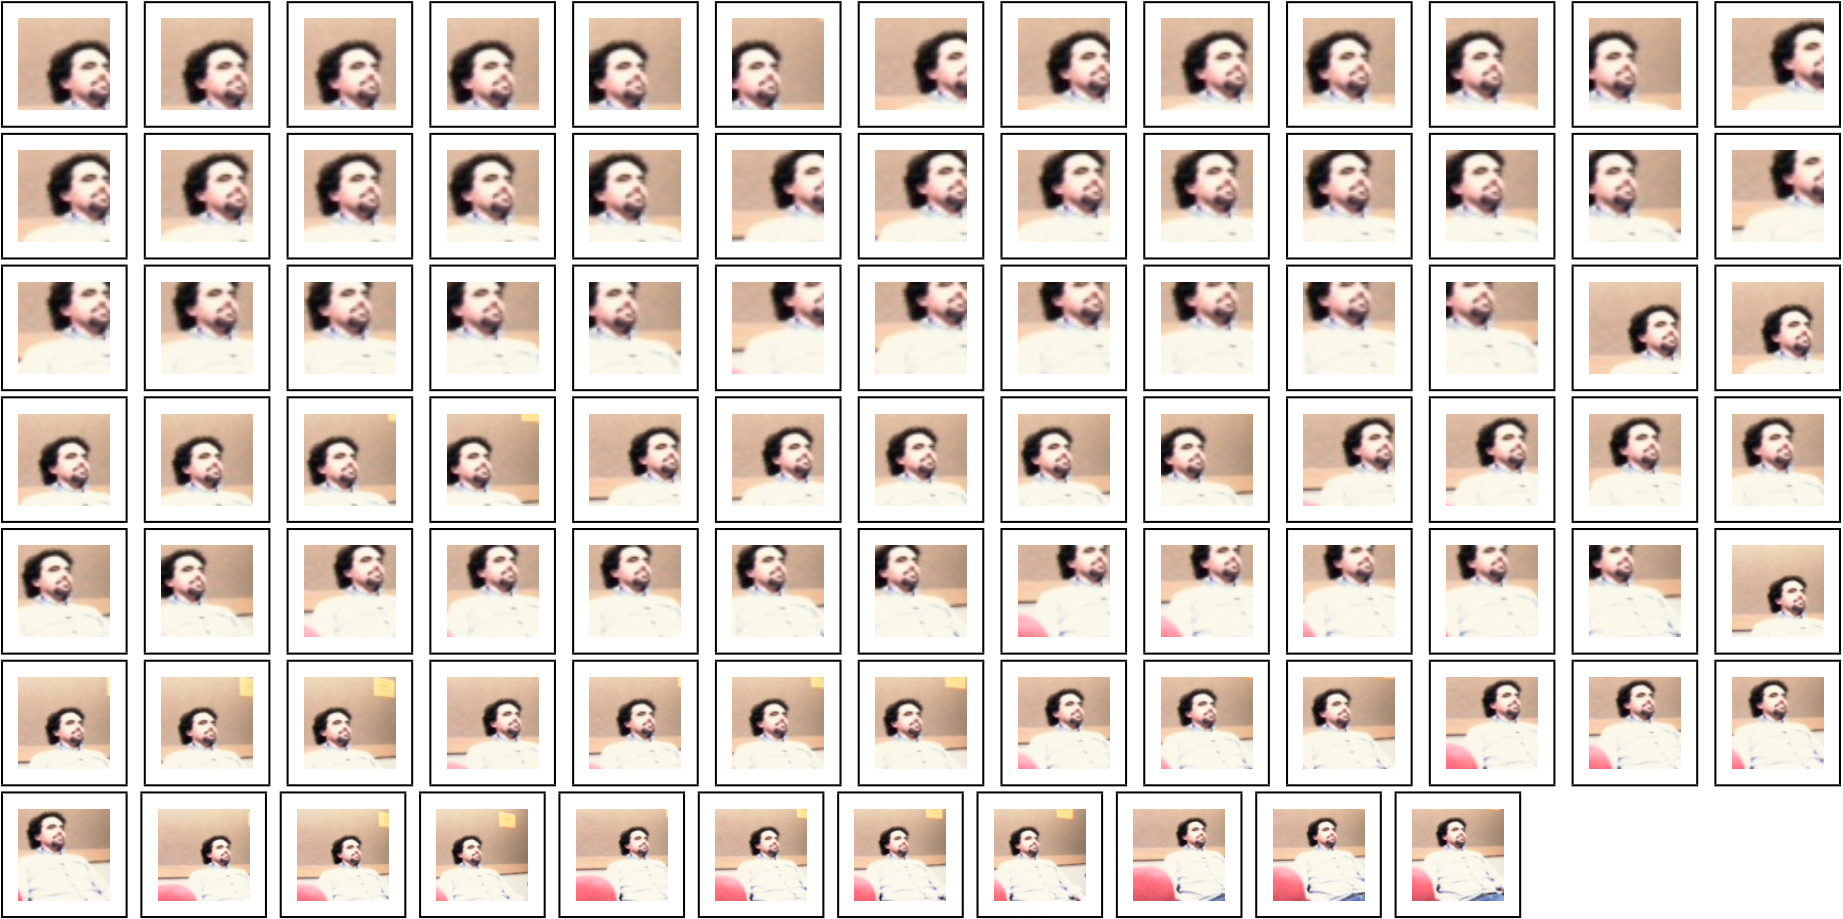
\includegraphics[width=1\textwidth]{windows.png}
% 		\end{center}
% 	\end{frame}


% 	\begin{frame}{Focus of work}
% 		% \begin{center}

% 			\begin{itemize}
% 				\item Object detection is an MIL problem
% 				\item MIL boost is introduced
% 				\item Use MIL cost functions in the Anyboost framework
% 				\item Solve problems associated with manual labelling
% 			\end{itemize}

% 			% In this paper, we acknowledge that object detection is innately a MIL
% 			% problem, and we introduce MIL boost, a boosting method that combines cost
% 			% functions from MIL literature with the Anyboost framework, to solve the
% 			% problems associated with manual labelling.
% 		% \end{center}
% 	\end{frame}


% 	\section{Anyboost}


% 	\begin{frame}{The Anyboost Framework}
% 		\begin{center}
% 			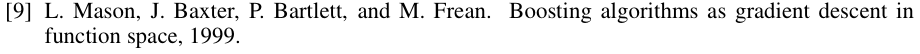
\includegraphics[width=1\textwidth]{anyboost-citation.png}

% 			The anyboost framwork views boosting as iterative gradient
% 			descent, where a cost functional is minimised over an inner
% 			product space.

% 			% \begin{itemize}
% 			% \end{itemize}
% 		\end{center}
% 	\end{frame}

	
% 	% show a crop of the first page

% 	% consider showing the table

% 	\section{MIL}

% 	\begin{frame}{Multiple Instance Learning}
% 		\begin{itemize}
% 			\item Training examples are positive or negative
% 			\item Group training examples into bags
% 			\item Bag labels are a logical \(\operatorname{OR}\) of bag contents
% 			\item Allows the classifier to identify the best training examples in each bag
% 		\end{itemize}
% 	\end{frame}


% 	\section{MIL and Boosting}

% 	\subsection{Noisy-OR Boost}

% 	\begin{frame}{Noisy-OR Boost}
% 		% \begin{center}
% 			Let $i$ index bags, and $j$ index examples.

% 			Score of example \(x_{ij}\):
% 			\[y_{ij} = C(x_{ij})\]
% 			is a weighted sum of weak classifiers:
			
% 			\[C(x_{ij}) = \sum_t{\lambda_t c^t(x_{ij})}\]
			
% 			where \(c(x_{ij}) \in \{-1, +1\}\).

% 			Define a probability of an example being positive using the logistic function:
% 			\[p_{ij} = \frac{1}{1 + \operatorname{exp}(-y_{ij})} \in [0, 1] \]

% 		% \end{center}
% 	\end{frame}


% 	\begin{frame}{Bag probability and classifier likelihood}
% 		% \begin{center}

% 		Use this to define the probability that a bag is positive using a `noisy OR' % TODO: cite!
		
		
		
% 		\[p_{i} = 1 - \prod_{j\in i}(1 - p_{ij})\]

% 		\[p_i = 1 - P(\text{all examples are negative})\]
% 		\[p_i = P(\text{at least one example is positive})\]


% 		Define likelihood assigned to a set of training bags.
% 		(likelihood that the classifier is correct)
% 		\[L(C) = \prod_{i}{p_i}^{t_i}(1 - p_{i})^(1-t_i)\]
% 		where \(t_i \in \{0, 1\} \) is the label of bag \(i\).

% 		% \end{center}
% 	\end{frame}
	
% 	\begin{frame}{}
% 		% \begin{center}

% 		Weight each example using the derivative of the cost function with respect to the score
		
% 		\[ \frac{\partial \operatorname{log} L(C)}{\partial y_{ij}} = w_{ij} = \frac{t_i - p_i}{p_i}p_{ij} \]
		
% 		e.g. if increasing the score increases the probability of the bag being positive, then $w_{ij}$ is positive. Thus, the sign of $w_{ij}$ determines the example label.

% 		% \end{center}
% 	\end{frame}
	
	
% 	\begin{frame}{}
% 		% \begin{center}

% 			Each round of boosting is a search for a classifier which maximizes 
% 			\[\sum_{ij} c(x_{ij})w_{ij}\]

% 			where \(c(x_{ij}) \in \{-1, +1\}\).
			

% 			\(\lambda_t\) is determined by to maximize \(\operatorname{log} L(C + \lambda_tc_t)\)

% 		% \end{center}
% 	\end{frame}

% 	\subsection{ISR Boost}

% 	\begin{frame}{ISR Boost}
% 		% \begin{center}
% 			ISR boost was also investigated:

% 			\(\chi_{ij} = \operatorname{exp}(y_{ij})\), \(S_i = \sum_{j \in i}{\chi_{ij}}\), and \(p_i = \frac{S_i}{1 + S_i}\). \\

% 			$\chi_{ij}$ can be treated as the likelihood of an object occuring in example $ij$.

% 			$S_i$ can be interpreted as a likelihood ratio that bag i is positive. \\

% 			Weights are slightly different
% 			\[ \frac{\partial \operatorname{log} L(C)}{\partial y_{ij}} = w_{ij} = (t_i - p_i)\frac{\chi_{ij}}{\sum_{j \in i}{\chi_{ij}}} \]
% 		% \end{center}
% 	\end{frame}


% 	\subsection{Comparison of MIL cost functions}

% 	\begin{frame}{Major differences}
% 		\begin{center}

% 			\begin{itemize}
% 				\item Examples explicitly compete for weight (weak experimental evidence, but might cause only one example in each bag to be labelled positive)

% 				\item Negative examples also compete for weight. Could cause problems, since negative examples greatly outnumber positive examples
% 				(Noisy OR criteria treats all negative examples as independent).

% 			\end{itemize}
% 		\end{center}
% 	\end{frame}


% 	\section{Application}

% 	\begin{frame}{Detection Cascade}
% 		\begin{itemize}
% 			\item Important for speed
% 			\item Retrain initial classifier after initial training
% 			\item Repeat for additional performance gains
% 		\end{itemize}

% 		% \begin{center}
% 			% after training the full classifier, retrain the first few weak classifiers to have a very low false negative rate on the examples labeled positive by the full classifier
% 		% \end{center}
% 	\end{frame}

% 	\begin{frame}{Dataset collection}
% 		% \begin{center}
% 			\begin{itemize}
% 				\item Sliding window, between 10000 and 100000 windows in a training image
% 				\item Each window is an example
% 				\item 8 videos in different conference rooms
% 				\item 	1856 images sampled from the set of videos
% 				\item 	detectors trained on 7 videos, and tested on the remaining one
% 				\item 	12364 visible people in the images, each manually labeled by drawing a rectangle around the head of each person
% 			\end{itemize}
% 		% \end{center}
% 	\end{frame}	

% 	\begin{frame}{Positive window and bag generation}
% 		% \begin{center}
% 			\begin{itemize}
% 				\item Windows are automatically labelled based on the manually labelled heads
% 				\item Tighter bounds are used for Adaboost
% 				\item One bag for each labelled head, which contains positive windows that overlap the head, and one negative bag for each image
% 			\end{itemize}
% 		% \end{center}
% 	\end{frame}

% 	\begin{frame}{Positive window and bag generation}
% 		\begin{center}
% 			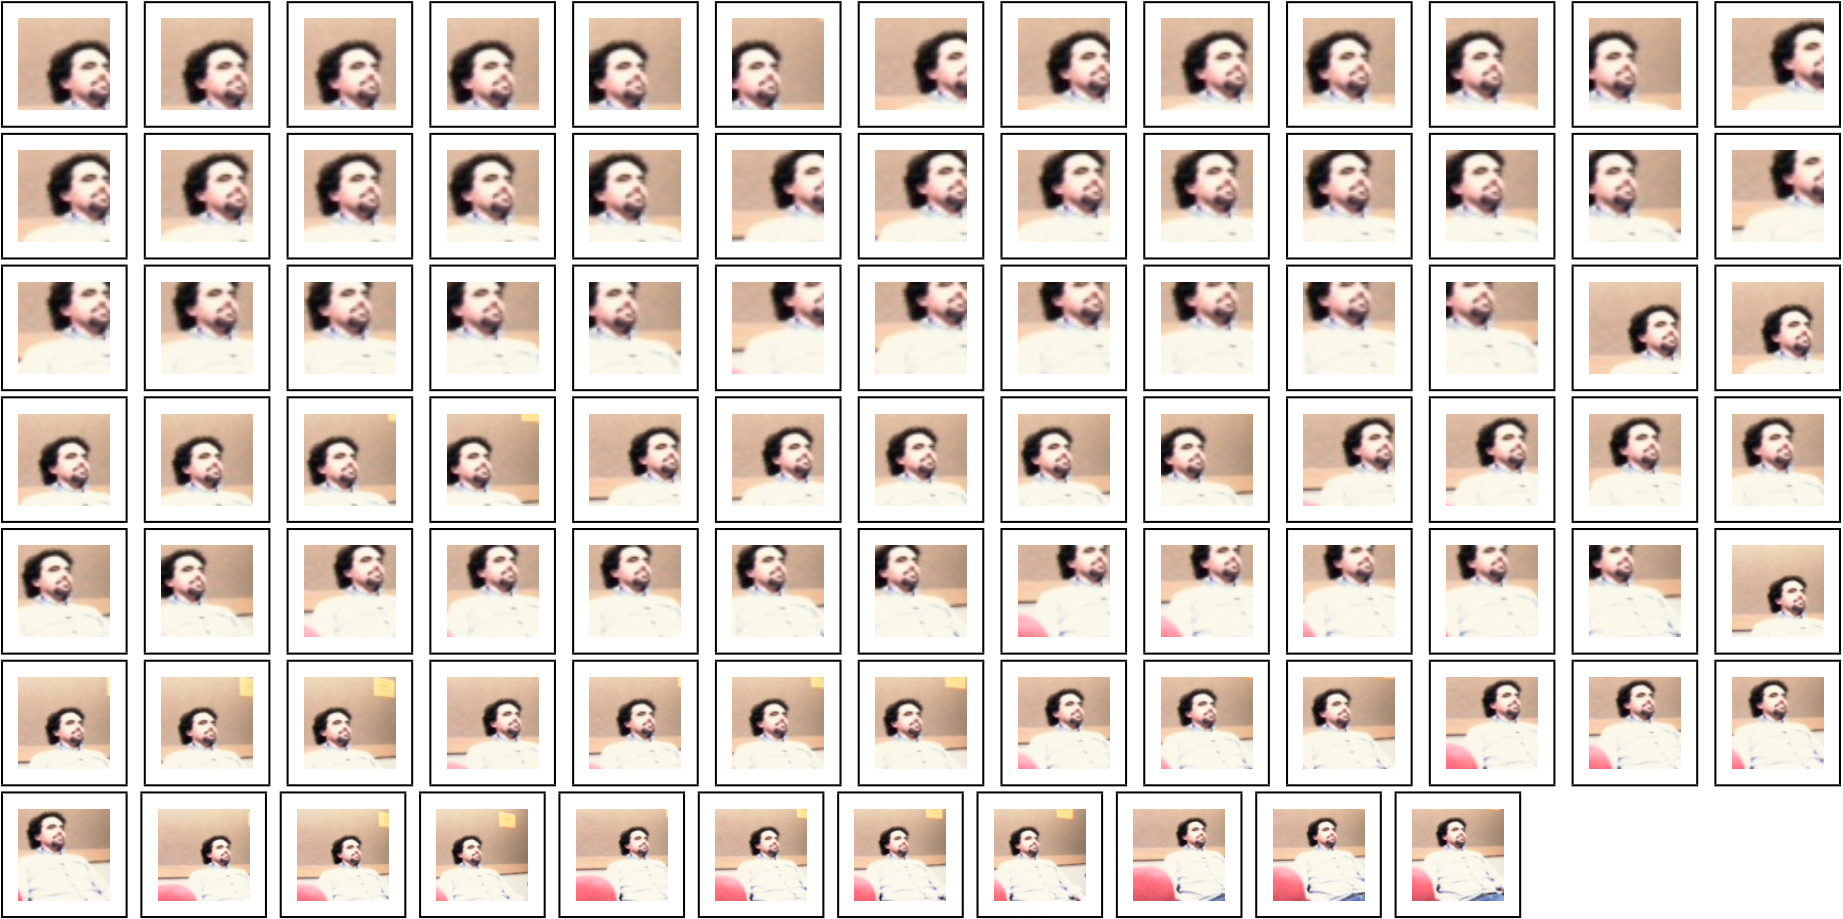
\includegraphics[width=1\textwidth]{windows.png}
% 		\end{center}
% 	\end{frame}


% 	\begin{frame}{Experiment description}
% 		% \begin{center}
% 			\begin{itemize}
% 				\item 	Learning performed on close to 30million subwindows of the 1856 images
% 				\item 	Monochrome and two `features images' are used
% 					\begin{itemize}
% 						\item Difference from the running mean image (something like background subtraction)
% 						\item Temporal variance over longer time scales
% 					\end{itemize}
% 				\item 	set of 2654 rectangle filters are used for training
% 				\item 	60 filters learned in each experiment. (optimal filter and threshold selected in each round

% 			\end{itemize}
% 		% \end{center}
% 	\end{frame}


% 	% \begin{frame}{Experiment results}
% 	% 	\begin{center}
% 	% 		\begin{itemize}
% 	% 			\item adaboost compared with both types of MIL boost
% 	% 		\end{itemize}
% 	% 	\end{center}
% 	% \end{frame}


% 	% \begin{frame}{Definition of positive examples}
% 	% 	\begin{itemize}
% 	% 		\item Examples 
% 	% 		\item for MIL: one bag for each labelled head, which contains positive windows that overlap the head, and one negative bag for each image
% 	% 	\end{itemize}
% 	% \end{frame}


% 	\begin{frame}{Real and corrupted ground truth}
% 		%\begin{center}
% 		Two training datasets were tested:
% 			\begin{itemize}
% 				\item The original set
% 				\item Corrupted ground truth (uniform random shift of each box).
% 			\end{itemize}
% 		%\end{center}
% 	\end{frame}


% 	\begin{frame}{ROC Curves}
% 		\begin{center}
% 			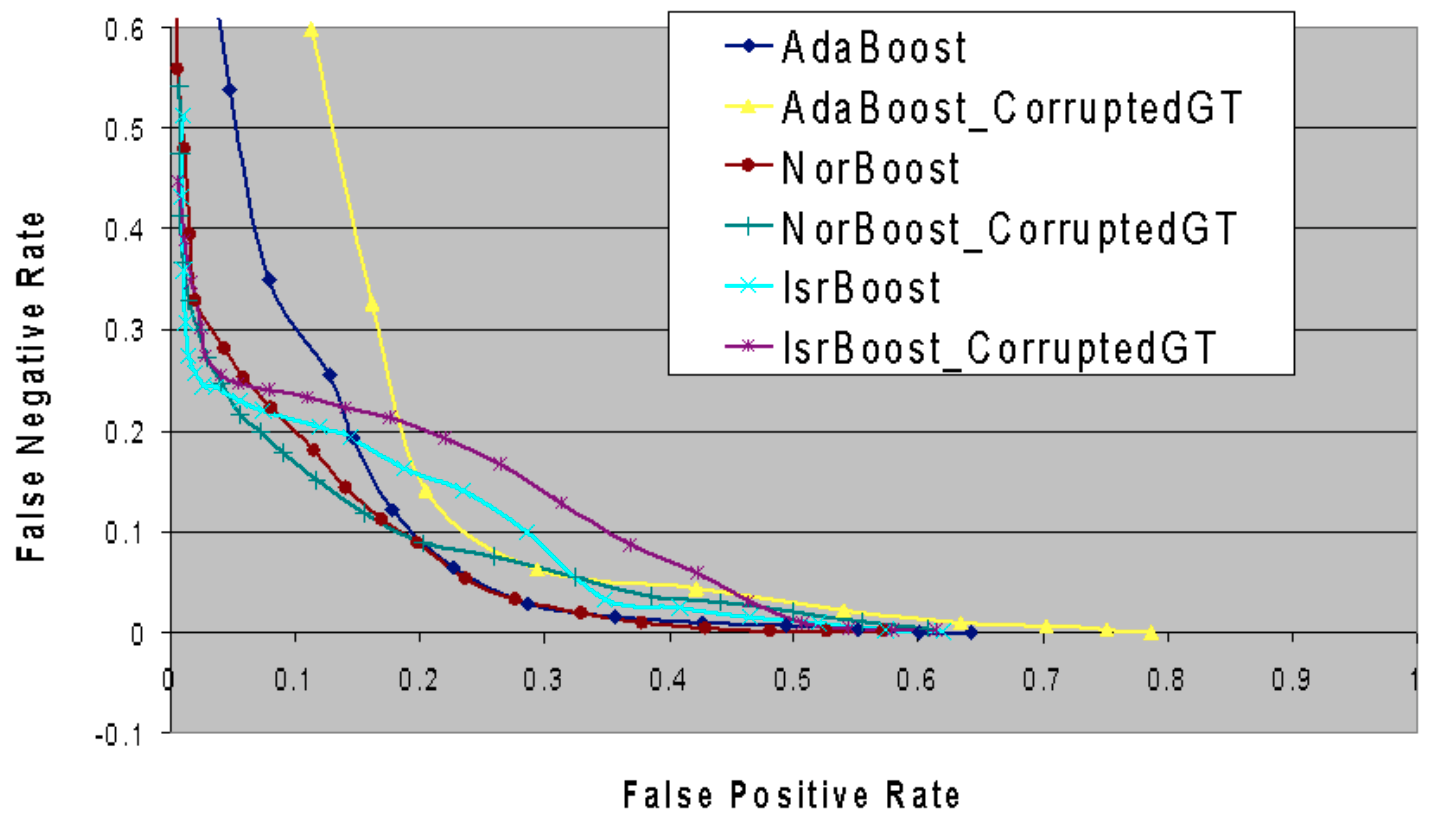
\includegraphics[width=1\textwidth]{roc-curves.png}
% 		\end{center}
% 	\end{frame}


% 	\begin{frame}{Typical performance}
% 		\begin{center}
% 			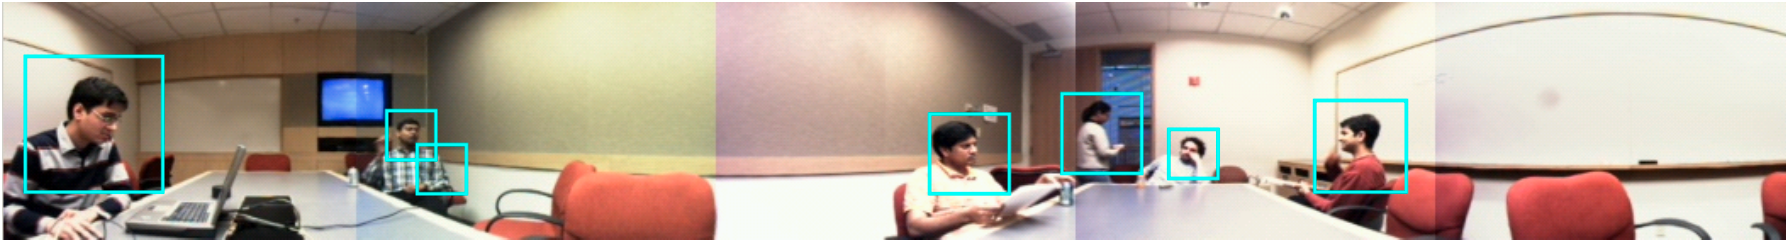
\includegraphics[width=1\textwidth]{results-image.png}
% 		\end{center}
% 	\end{frame}


% 	\begin{frame}{Conclusion}
% 		\begin{center}
% 			Using MILBoost reduced label noise and improves performance over standard Adaboost.
% 		\end{center}
% 	\end{frame}

% \end{document}

